\documentclass[10pt,letterpaper]{article}
\usepackage{amsmath}
\usepackage{amssymb}
\usepackage{fancyhdr}
\usepackage[bottom=1in, top=1in, left=1in, right=1in]{geometry}
\usepackage{graphicx}
\usepackage{here}
\usepackage[T1]{fontenc}
\DeclareGraphicsExtensions{.pdf,.png,.jpg}

\pagestyle{fancy}
\setlength{\headheight}{.5in}
\setlength{\parindent}{0in}

\begin{document}

\rhead{
          Paul Boschert\\
          09/04/2015\\
          CSCI 5622 - Machine Learning: Homework 1 Analysis \\
      }


\textbf{\textit{1)}}
In knn.py, as the number of training points increases, the accuracy rises.  This appears to be the case regardless of the $k$.  When the minimum number of training points is used ($k$), the accuracy is very poor.  But when the entire dataset is used for training, the accuracy rises to $~0.97$.  It's interesting to see that the accuracy rises almost exponentially until the number of training points rises to $~ 4000$, then it stays about the same.  See Figure \ref{fig:accuracyVsTrainingPoints} for more details.\\
\begin{figure}[h]
  \centering
  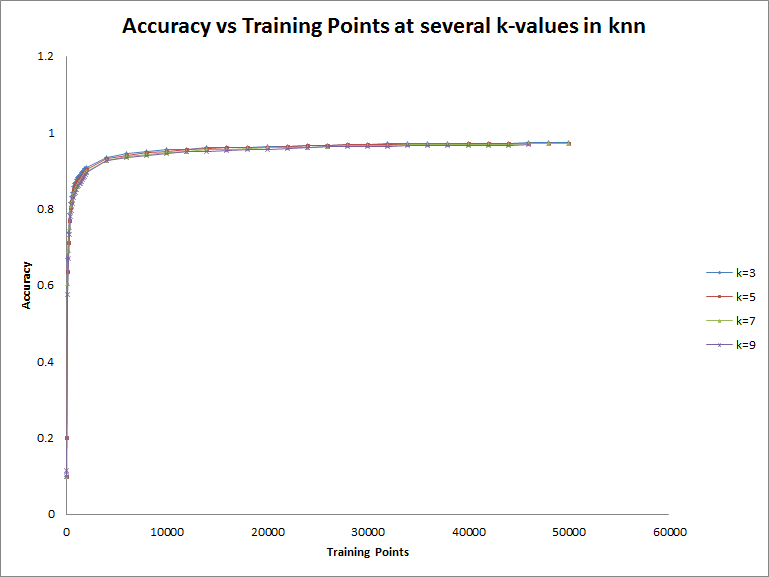
\includegraphics[scale=.4]{accuracyVsTrainingPoints}
  \caption{The relationship of accuracy and training points}
  \label{fig:accuracyVsTrainingPoints}
\end{figure}

\textbf{\textit{2)}}
$k$ has a much more interesting relationship to the accuracy.  Generally when $k$ is too small, the accuracy is poor.  Also when $k$ is too large, the accuracy is poor.  The $k$ that corresponds to the best accuracy is some where in the middle.  When using 10,000 training points, the highest accuracy corresponds to a $k$ of 3.  See Figure \ref{fig:accuracyVsK} for more details.\\
\begin{figure}[h]
  \centering
  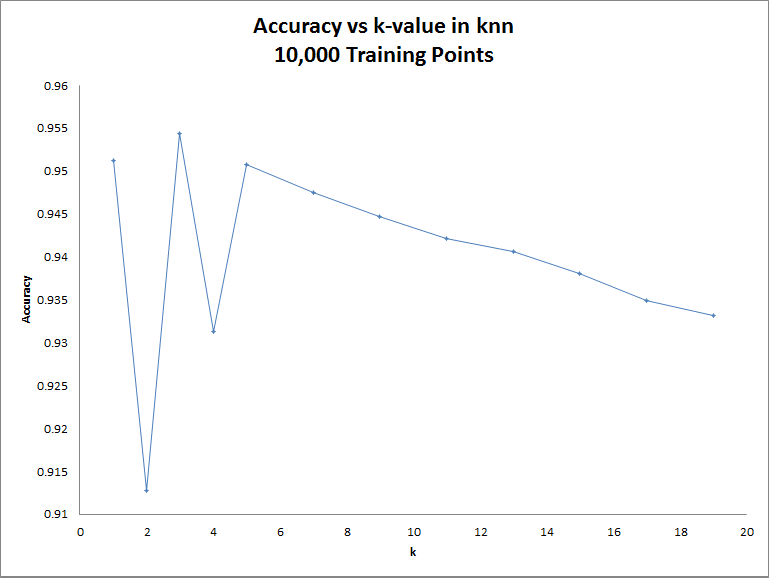
\includegraphics[scale=.4]{accuracyVskValue}
  \caption{The relationship of accuracy and k-value.}
  \label{fig:accuracyVsK}
\end{figure}



\textbf{\textit{3)}}
For this question, I used the entire data set and a $k$ of 3.  This has the best accuracy.  The confusion matrix clearly shows the most hits along the diagonal where the guess is the same as the answer.  Outside of the diagonal are the mis-classifications.  The top three mis-classificiations are:\\
4 classified as 9: 19 times\\
8 classified as 5: 18 times\\
2 classified as 7: 18 times

\end{document}

